\chapter{Практические задания}
\section{Разработать программу "Телефонный справочник" (ЛР №1, часть 1).}
\begin{lstlisting}[caption=Задание 1]
include "lab_telephone.inc"
	
domains
	name = string
	phone = string
	
predicates
	phone(name, phone).
	
clauses
	phone(ellen, "367890").
	phone(john, "475910").
	phone(tom, "458457").
	phone(eric, "483557").
	phone(mark, "104857").
	
goal
	phone(mark, X).
\end{lstlisting}

\section{Задание 2 (ЛР №1, часть 2)}
\textbf{Задание:} составить программу -- базу знаний, с помощью которой можно определить, например, множество студентов, обучающихся в одном ВУЗе и их телефоны. Студент может одновременно обучаться в нескольких ВУЗах. Привести примеры возможных вариантов вопросов и варианты ответов (не менее 3-х). Описать порядок формирования ответа.
\newpage
\begin{lstlisting}[basicstyle=\footnotesize]
include "lab_telephone.inc"

domains
	id_university = integer.
	name_university = string.
	city_university = string.
	
	id_student = integer.
	surname_student = string.
	name_student = string.
	phone_number = string.

predicates
	phone(surname_student, phone_number).
	student(id_student, surname_student, name_student).
	university(id_university, name_university, city_university).
	
	education(id_student, id_university).
	
	from_one_university_info(name_university, surname_student,
	name_student, phone_number).
	education_info(surname_student, name_university).

clauses
	phone("Pavlov", "+7(934)245-34-12").
	phone("Ivanov", "+7(924)056-78-34").
	phone("Dremin", "+7(984)874-91-23").
	phone("Agafonova", "+7(945)012-85-93").
	phone("Voronina", "+7(912)395-03-04").
	phone("Abrikosova", "+7(934)812-38-47").
	
	student(1, "Pavlov", "Semen").
	student(2, "Ivanov", "Vladimir").
	student(3, "Dremin", "Ilya").
	student(4, "Agafonova", "Julia").
	student(5, "Voronina", "Sofia").
	student(6, "Abrikosova", "Elena").
	
	university(1, "BMSTU", "Moscow").
	university(2, "ITMO", "St. Petersburg").
	university(3, "SFU", "Krasnoyarsk").

	education(1, 3).
	education(2, 1).
	education(3, 2).
	education(4, 3).
	education(5, 3).
	education(6, 1).
	education(1, 3).
	education(1, 2).

	from_one_university_info(Name_university, Surname, Name_student, 
							Phone_number
							) :- education(StudentID, UniversityID),
							     student(StudentID, Surname, Name_student),
							     university(UniversityID, Name_university, _),
								 phone(Surname, Phone_number).

	education_info(Surname, 
				   Name_university) :- education(StudentID, UniversityID),
									   student(StudentID, Surname, _),
									   university(UniversityID, Name_university, _).
goal
	%student(Id, Name, Surname).
	%education_info("Pavlov", Name_university).
	%Answers:
	%Name_university=SFU
	%Name_university=BMSTU
	%Name_university=ITMO
	
	%from_one_university_info("SFU", Surname, Name_student, Phone_number).
	%Answers:
	%Surname=Pavlov, Name_student=Semen, Phone_number=+7(934)245-34-12
	%Surname=Agafonova, Name_student=Julia, Phone_number=+7(945)012-85-93
	%Surname=Voronina, Name_student=Sofia, Phone_number=+7(912)395-03-04
\end{lstlisting}

\chapter{Задание №3 (ЛР2, часть 1)}
\textbf{Задание:} составить программу, объединив в ней информацию-знания.
\begin{itemize}
	\item \textbf{<<Телефонный справочник>>}: Фамилия, №тел, Адрес -- структура (Город, Улица, №дома, №кв);
	\item \textbf{<<Автомобили>>}: Фамилия\_владельца, Марка, Цвет, Стоимость и др.;
	\item \textbf{<<Вкладчики банков>>}: Фамилия, Банк, счет, сумма, др.
\end{itemize}
Владелец может иметь несколько телефонов, автомобилей, вкладов (Факты).
Используя правила, обеспечить возможность поиска:
\begin{enumerate}
	\item 
	\begin{itemize}
		\item[a)] По номеру телефона найти: Фамилию, Марку автомобиля, Стоимость (может быть несколько).
		\item[b)] Используя сформированное в пункте a) правило, по №телефона найти только Марку автомобиля (автомобилей может быть несколько).
	\end{itemize}
	\item Используя простой, не составной вопрос: по Фамилии (уникальна в городе, но в разных городах есть однофамильцы) и Городу проживания найти: Улицу проживания, Банки, в которых есть вклады, и №телефона. 
\end{enumerate}
Для задания 1 и 2: для одного из вариантов ответов, и для a), и для b) описать словесно порядок поиска ответа на запрос, указав, как выбираются значения, и при этом для каждого этапа унификации, выписать подстановку -- наибольший общий унификатор и соответствующие примеры термов.
\begin{lstlisting}[basicstyle=\footnotesize]
include "lab_telephone.inc"

domains
	%phone
	surname = string
	phone_number = string
	city = string
	street = string
	house_number = integer
	flat_number = integer
	struct_address = address(city, street, house_number, flat_number)
	
	%cars
	car_brand = string
	car_color = string
	car_cost = integer
	
	%bank depositor
	bank_name = string
	bank_account = string
	account_cost = integer

predicates
	phone(surname, phone_number, struct_address).
	car(surname, car_brand, car_color, car_cost).
	bank_depositor(surname, bank_name, bank_account, account_cost).
	
	find_info_by_number(phone_number, surname, car_brand, car_cost).
	find_car_brand_by_number(phone_number, car_brand).
	find_info_by_surname_city(surname, city, phone_number, street, bank_name).
	find_info_by_brand_color(car_brand, car_color, surname, city, phone_number, bank_name).

clauses
	phone("Pavlov", "+7(934)245-34-12", 
		  address("Moscow", "St.1905 year", 20, 154)).
	phone("Pavlov", "+7(924)056-78-34", 
		  address("Moscow", "St.1905 year", 20, 154)).
	phone("Dremin", "+7(984)874-91-23", 
		  address("Moscow", "Tverskaya", 53, 26)).
	phone("Agafonova", "+7(934)812-38-47",
	      address("Moscow", "Bolshaya Dmitrovka", 7, 15)).
	phone("Agafonova", "+7(956)361-31-17",
		  address("Moscow", "Bolshaya Dmitrovka", 7, 15)).
	
	car("Pavlov", "Toyota Camry", "Silver", 1200000).
	car("Pavlov", "Honda Oddysey", "Black", 900000).
	car("Dremin", "Honda Oddysey", "Black", 900000).
	car("Dremin", "Ford Mustang", "Blue", 1800000).
	
	bank_depositor("Agafonova", "Sberbank", "0401-2535", 15000).
	bank_depositor("Agafonova", "Tinkoff", "1431-5836", 25000).
	bank_depositor("Dremin", "VTB", "9631-7521", 20000).
	bank_depositor("Pavlov", "Alpha", "9631-7521", 20000).
	
	find_info_by_number(Phone_number, Surname, Car_brand, 
						Car_cost) :- phone(Surname, Phone_number, _),
									 car(Surname, Car_brand, _, Car_cost).
	find_car_brand_by_number(Phone_number, 
							 Car_brand) :- find_info_by_number(Phone_number, _, 
															  Car_brand, _).
	find_info_by_surname_city(Surname, City, 
			Phone_number, Street, Bank_name) :- phone(Surname, Phone_number, 
													address(City, Street, _, _)),
	bank_depositor(Surname, Bank_name, _, _).
	
	find_info_by_brand_color(Car_brand, 
			Car_color, Surname, City, 
			Phone_number, Bank_name) :- car(Surname, Car_brand, Car_color, _),
										phone(Surname, Phone_number, 
											  address(City, _, _, _)), 
										bank_depositor(Surname, Bank_name, _, _).	 


goal
	%find_info_by_number("+7(984)874-91-23", Surname, Car_brand, Car_cost).
	%find_car_brand_by_number("+7(984)874-91-23", Car_brand).
	%find_info_by_surname_city("Dremin", "Moscow", Phone_number, Street, Bank_name).
	
	%find_info_by_brand_color("Honda Oddysey", "Black", Surname, City, Phone_number, Bank_name).  
\end{lstlisting}

Результаты ответов на вопрос:
\begin{lstlisting}[basicstyle=\footnotesize]
find_info_by_number("+7(984)874-91-23", Surname, Car_brand, Car_cost).	
Surname=Dremin, Car_brand=Honda Oddysey, Car_cost=900000
Surname=Dremin, Car_brand=Ford Mustang, Car_cost=1800000

find_car_brand_by_number("+7(984)874-91-23", Car_brand).
Car_brand=Honda Oddysey
Car_brand=Ford Mustang

find_info_by_surname_city("Agafonova", "Moscow", Phone_number, Street,
						  Bank_name).
Phone_number=+7(934)812-38-47, Street=Bolshaya Dmitrovka, Bank_name=Sberbank
Phone_number=+7(934)812-38-47, Street=Bolshaya Dmitrovka, Bank_name=Tinkoff
Phone_number=+7(956)361-31-17, Street=Bolshaya Dmitrovka, Bank_name=Sberbank
Phone_number=+7(956)361-31-17, Street=Bolshaya Dmitrovka, Bank_name=Tinkoff

find_info_by_surname_city("Agafonova", "Moscow", Phone_number, Street, 
						  Bank_name).
Surname=Dremin, City=Moscow, Phone_number=+7(984)874-91-23, Bank_name=VTB
\end{lstlisting} 

Ниже приведена таблица порядка поиска ответов для задания 1а):
\begin{figure}[H]
	\centering{
		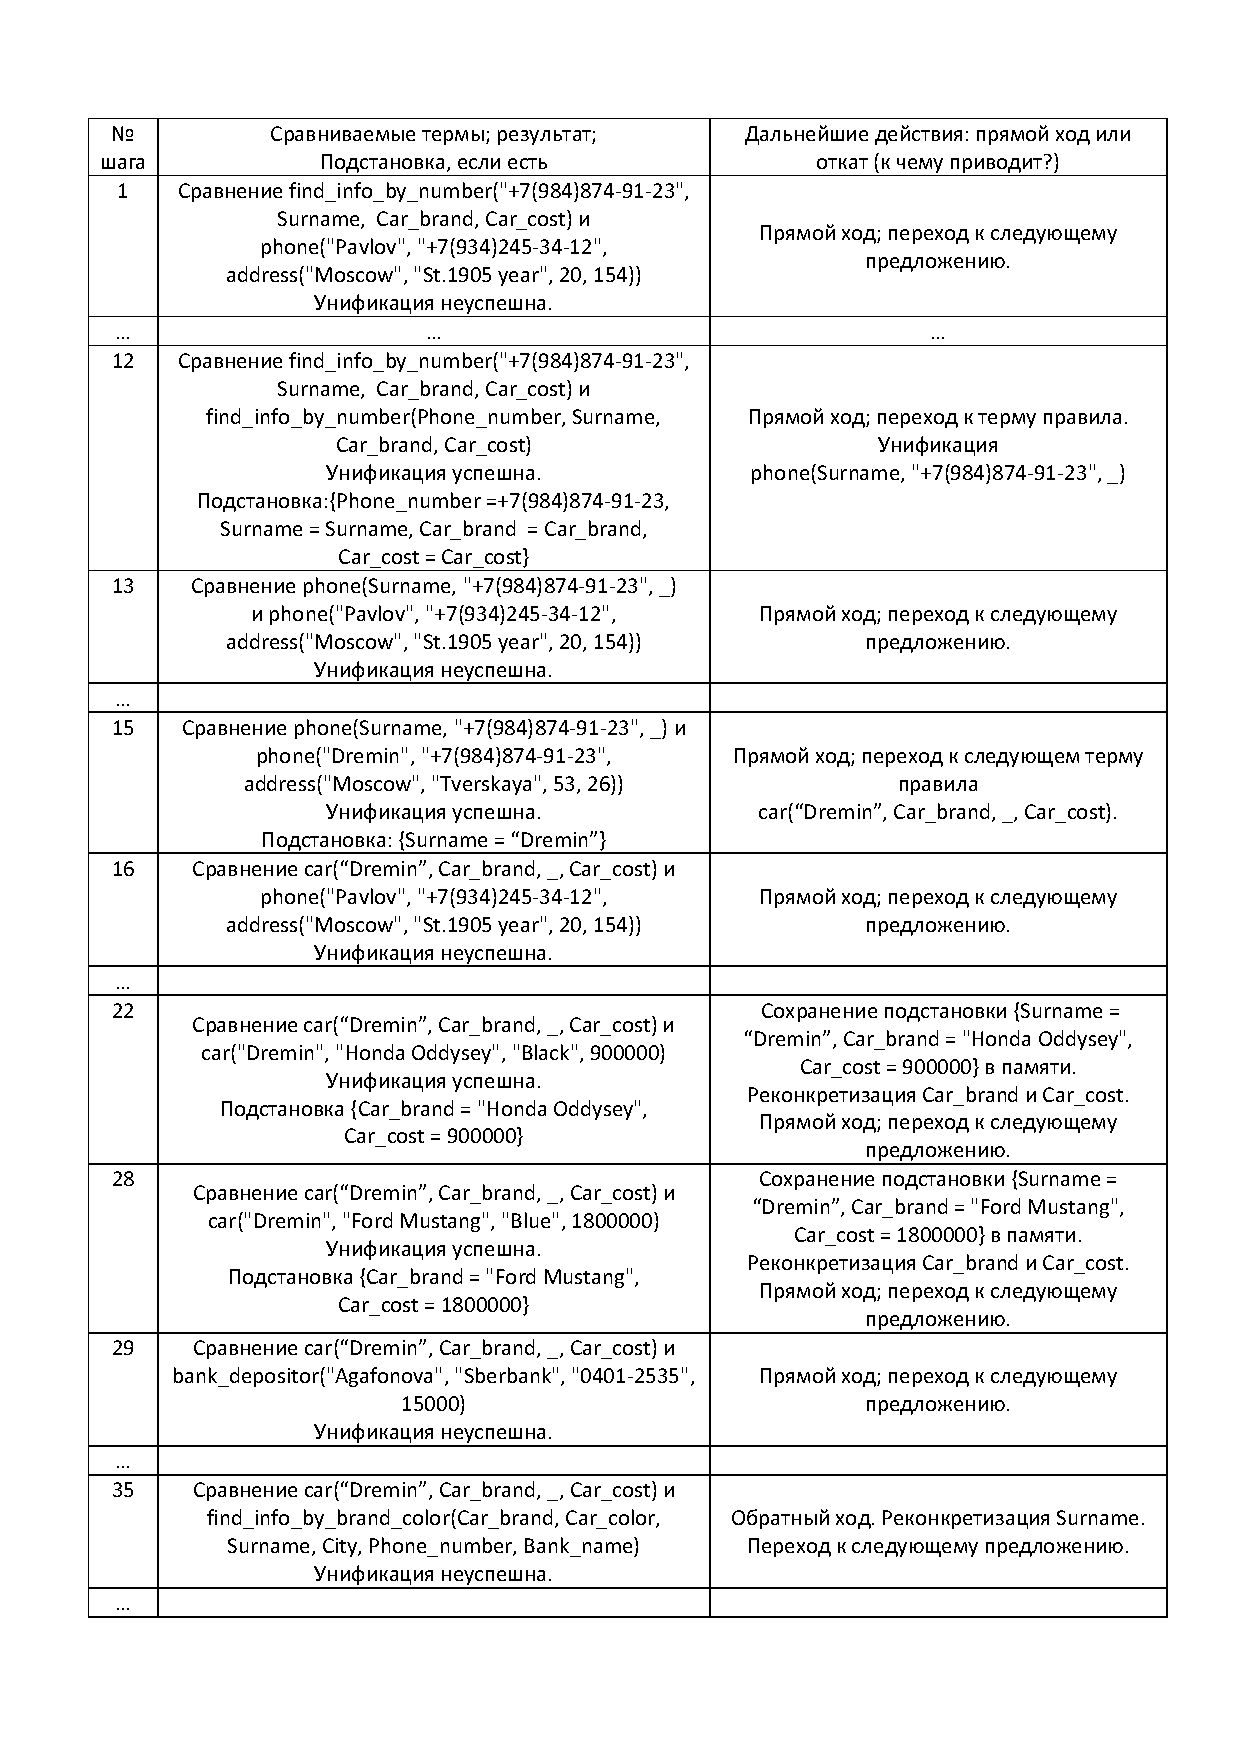
\includegraphics[scale=0.85]{images/table_1_1.pdf}
		\caption{Таблица порядка поиска ответов для задания 1а.}
		\label{png:1}}
\end{figure}

\begin{figure}[H]
	\centering{
		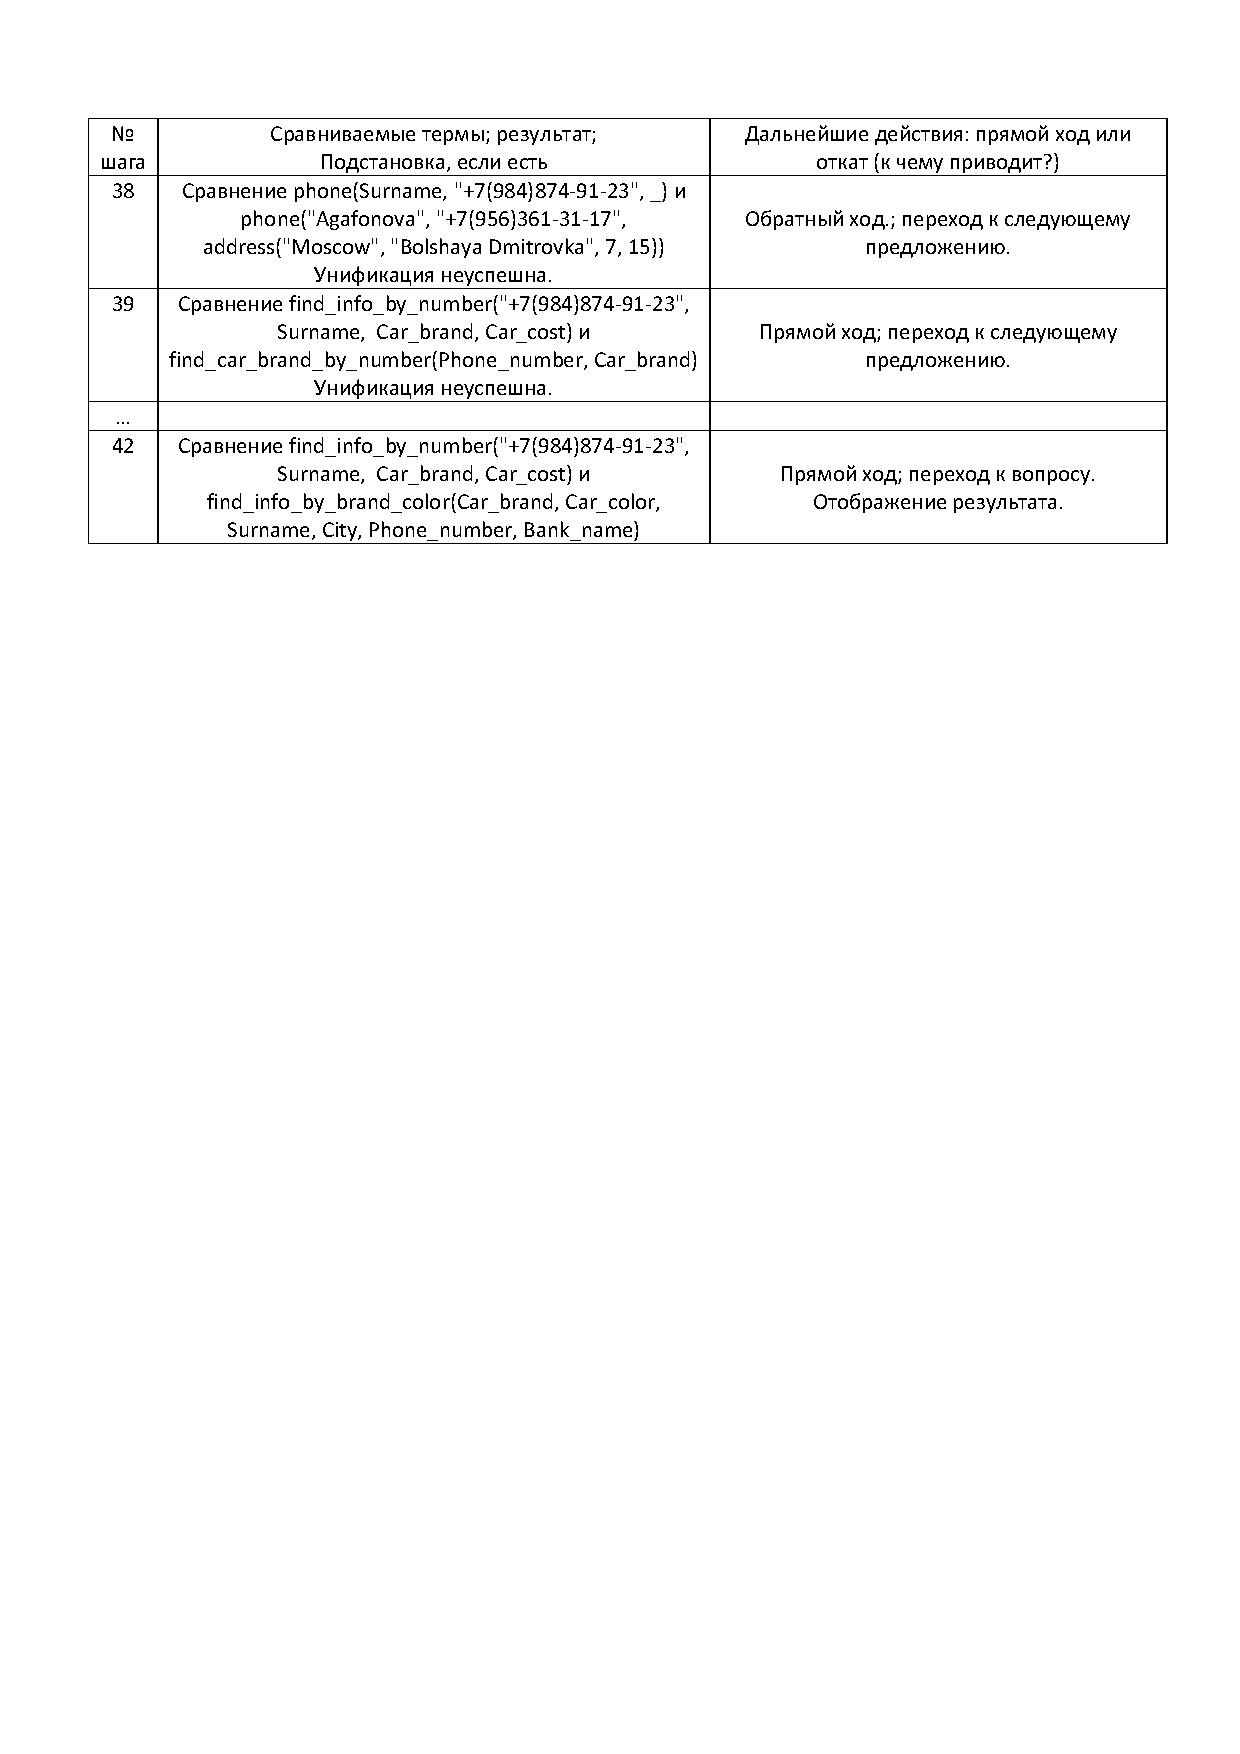
\includegraphics[scale=0.85]{images/table_1_2.pdf}
		\caption{Таблица порядка поиска ответов для задания 1а (продолжение).}
		\label{png:1}}
\end{figure}
Ниже приведена таблица порядка поиска ответов для задания 1b):
\begin{figure}[H]
	\centering{
		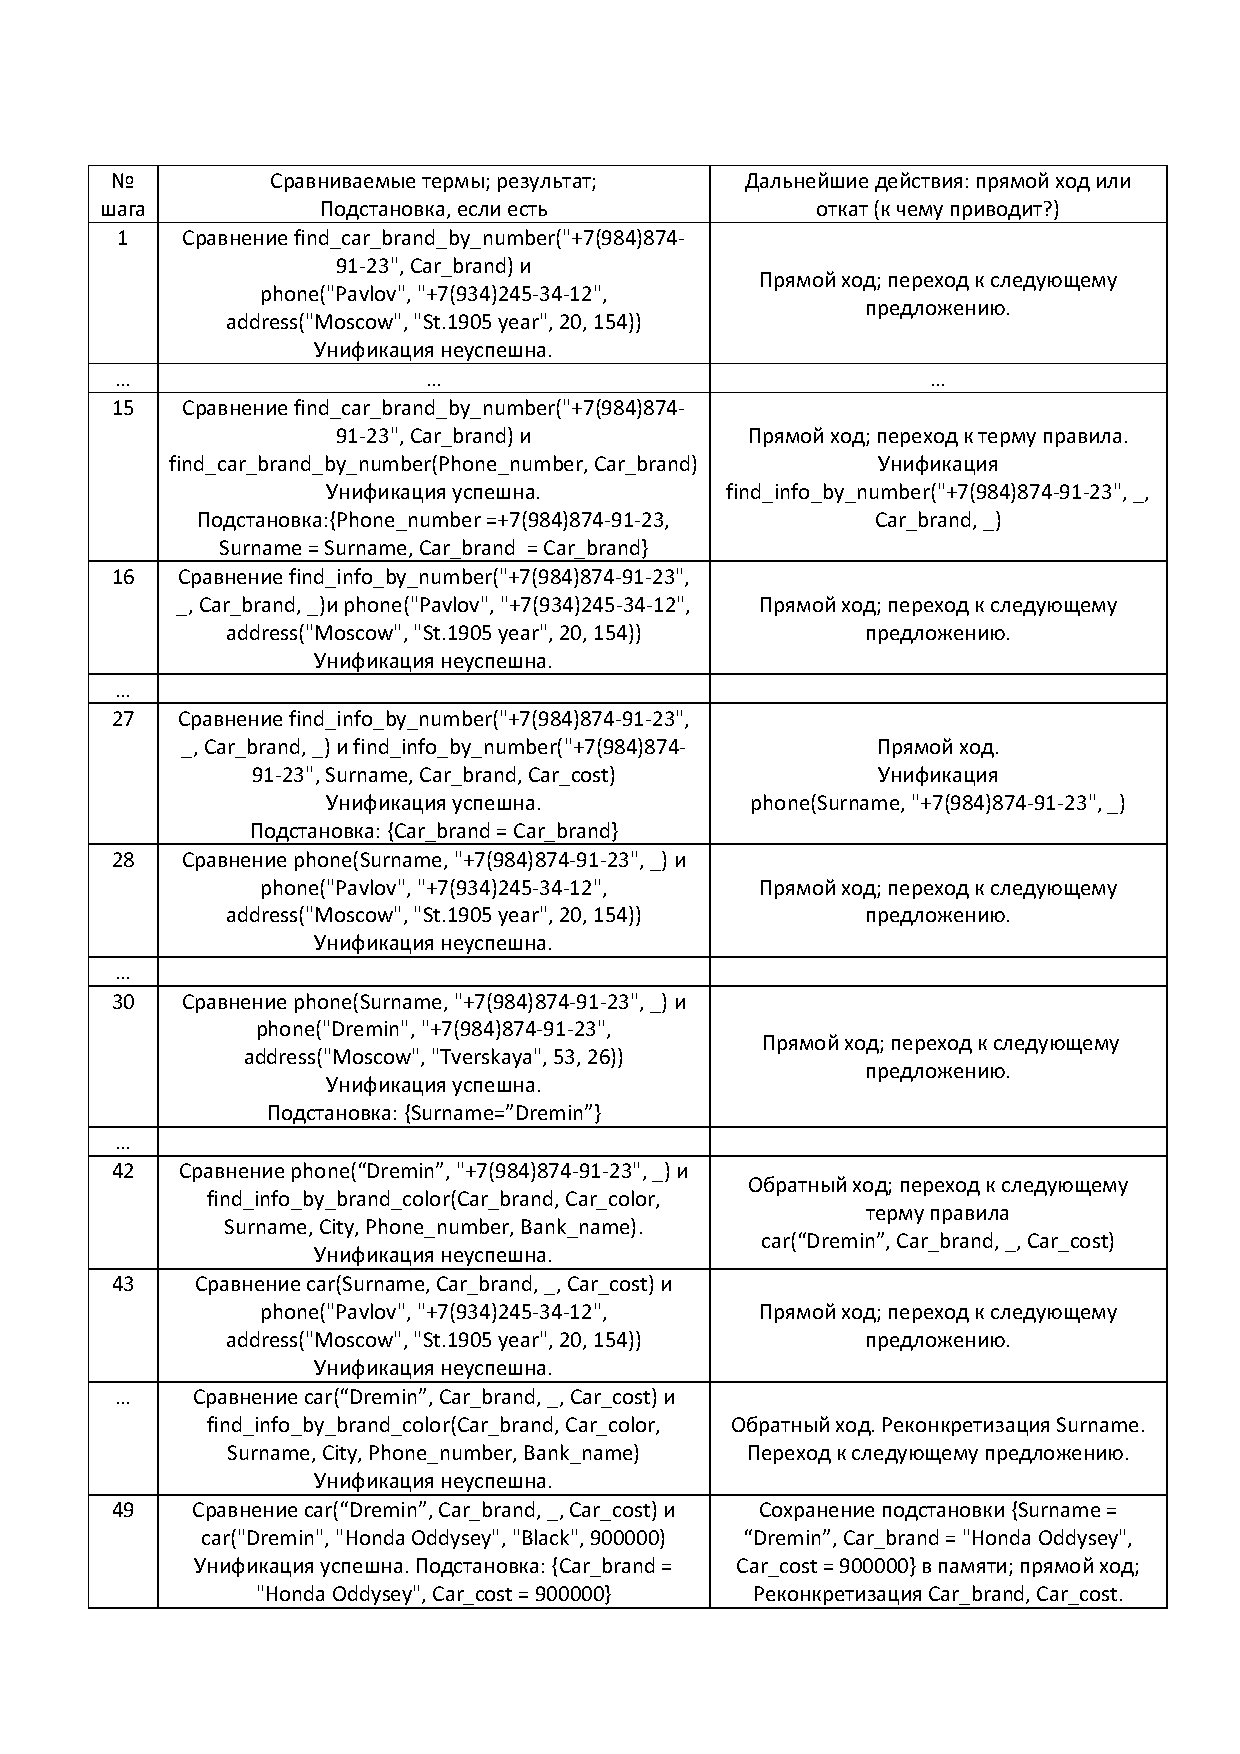
\includegraphics[scale=0.85]{images/table_2_1.pdf}
		\caption{Таблица порядка поиска ответов для задания 1b.}
		\label{png:1}}
\end{figure}

\begin{figure}[H]
	\centering{
		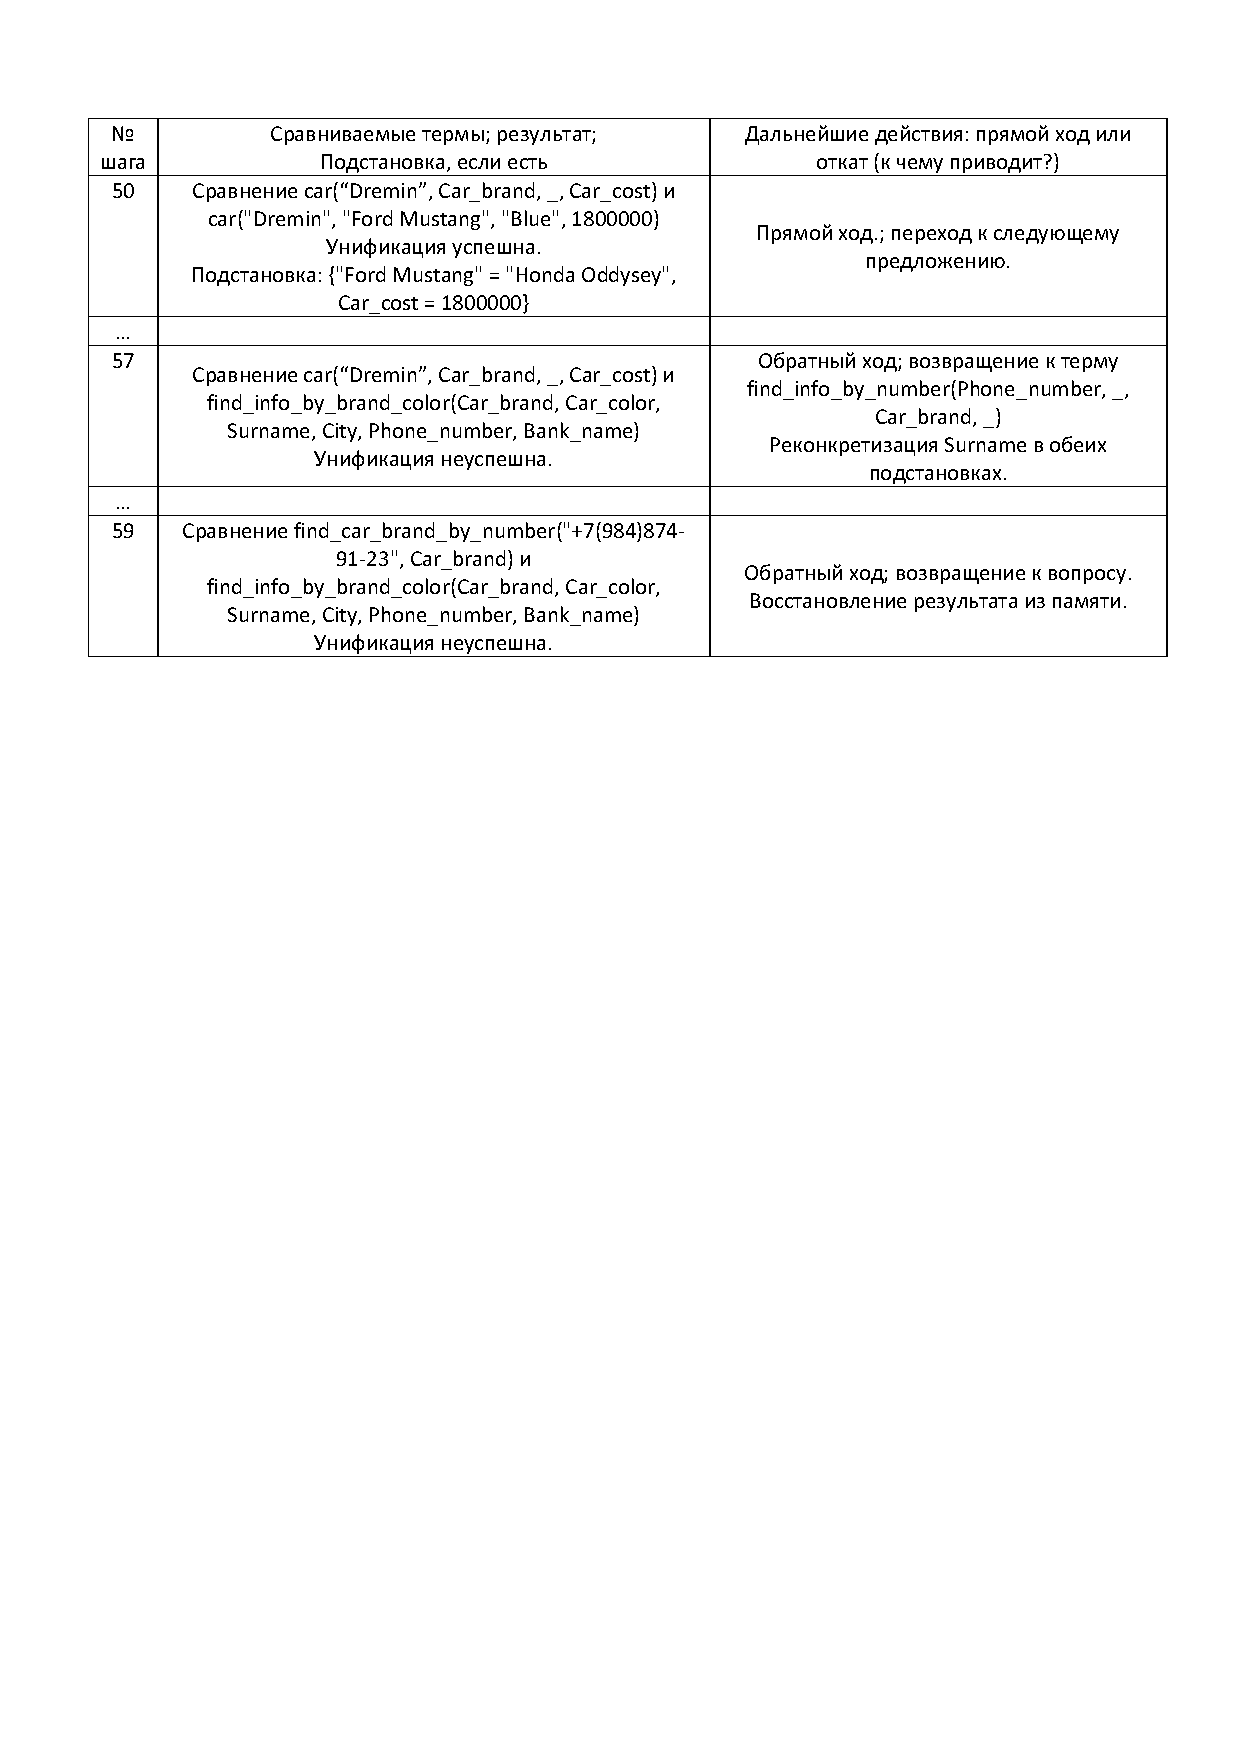
\includegraphics[scale=0.85]{images/table_2_2.pdf}
		\caption{Таблица порядка поиска ответов для задания 1b (продолжение).}
		\label{png:1}}
\end{figure}

\section{Задание №4 (ЛР2, часть 2)}
\textbf{Задание:} составить программу, объединив в ней информацию-знания.
\begin{itemize}
	\item \textbf{<<Телефонный справочник>>}: Фамилия, №тел, Адрес -- структура (Город, Улица, №дома, №кв);
	\item \textbf{<<Автомобили>>}: Фамилия\_владельца, Марка, Цвет, Стоимость и др.;
	\item \textbf{<<Вкладчики банков>>}: Фамилия, Банк, счет, сумма, др.
\end{itemize}
Владелец может иметь несколько телефонов, автомобилей, вкладов (Факты). В разных городах есть однофамильцы, водном городе фамилия уникальна.
Используя конъюнктивное правило и простой вопрос, обеспечить возможность поиска:

По Марке и Цвету автомобиля найти Фамилию, Город, Телефон и Банки, в которых владелец автомобиля имеет вклады.

Владельца может быть несколько (не более трех), один и ни одного.
\begin{enumerate}
	\item Для каждого из трех вариантов подробно описать порядок формирования ответа в виде таблицы. При этом указать -- отметить моменты очередного запуска алгоритма унификации и полный результат его работы. Обосновать следующий шаг работы системы. Выписать унификаторы -- подстановки. Указать моменты, причины и результат отката, если он есть.
	\item Для случая нескольких владельцев (2-х).
	Приведите пример (таблицы) работы системы при разных порядках следования в БЗ процедур, и знаний в них (<<Телефонный справочник>>, <<Автомобили>>, <<Вкладчики банков>> или <<Автомобили>>, <<Вкладчики банков>>, <<Телефонный справочник>>). Сделать вывод: одинаковы ли множество работ и объем в разных случаях.
	\item Оформите 2 таблицы, демонстрирующие порядок работы алгоритма унификации вопроса и подходящего заголовка правила (для двух случаев из пункта 2) и укажите результаты его работы: ответ и побочный эффект.
\end{enumerate}

Вопрос данного задания был добавлен в предыдущем листинге (см листинг).

Ниже приведена таблица порядка поиска ответов для задания 1):
\begin{figure}[H]
	\centering{
		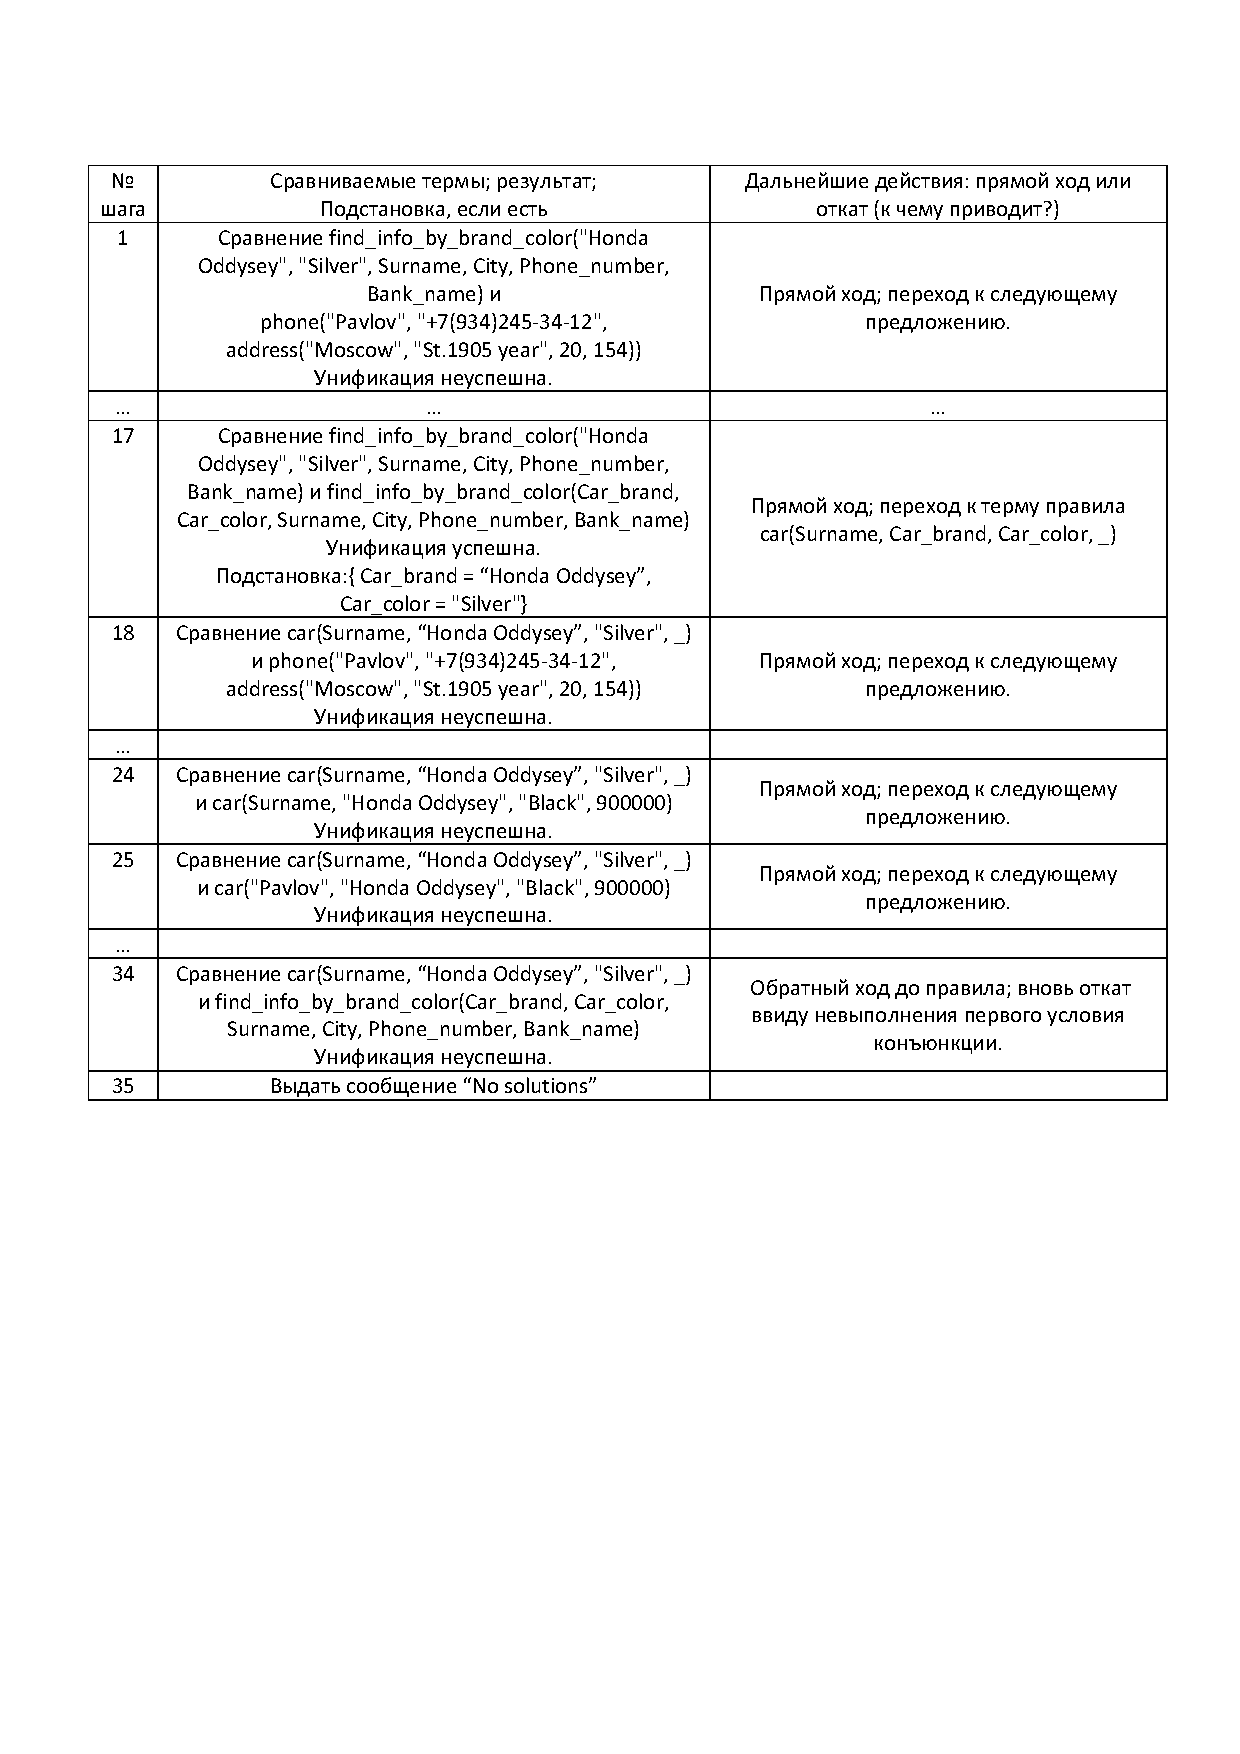
\includegraphics[scale=0.85]{images/table_2_3.pdf}
		\caption{Таблица порядка поиска ответов для задания никто не найден.}
		\label{png:1}}
\end{figure}

\begin{figure}[H]
	\centering{
		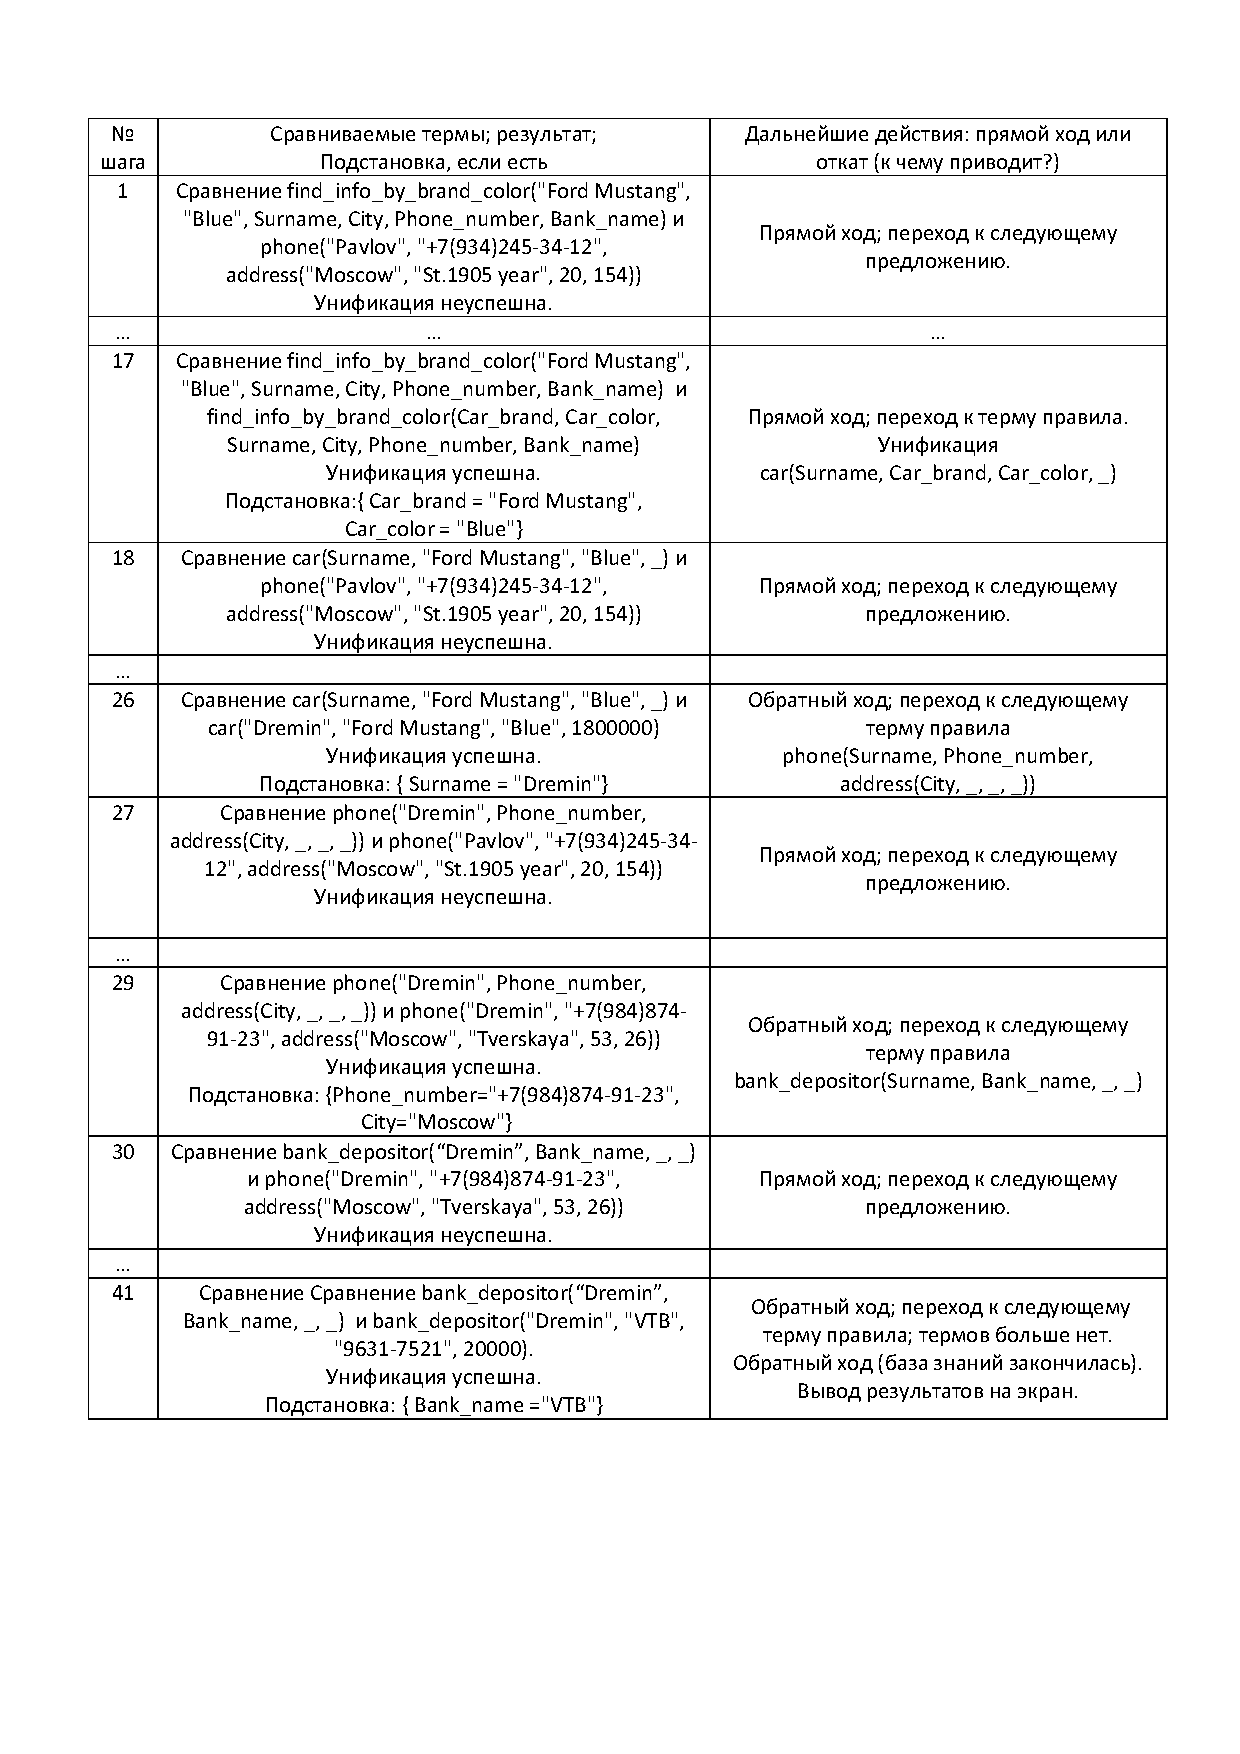
\includegraphics[scale=0.85]{images/table_2_4.pdf}
		\caption{Таблица порядка поиска ответов для задания найден один.}
		\label{png:1}}
\end{figure}

\begin{figure}[H]
	\centering{
		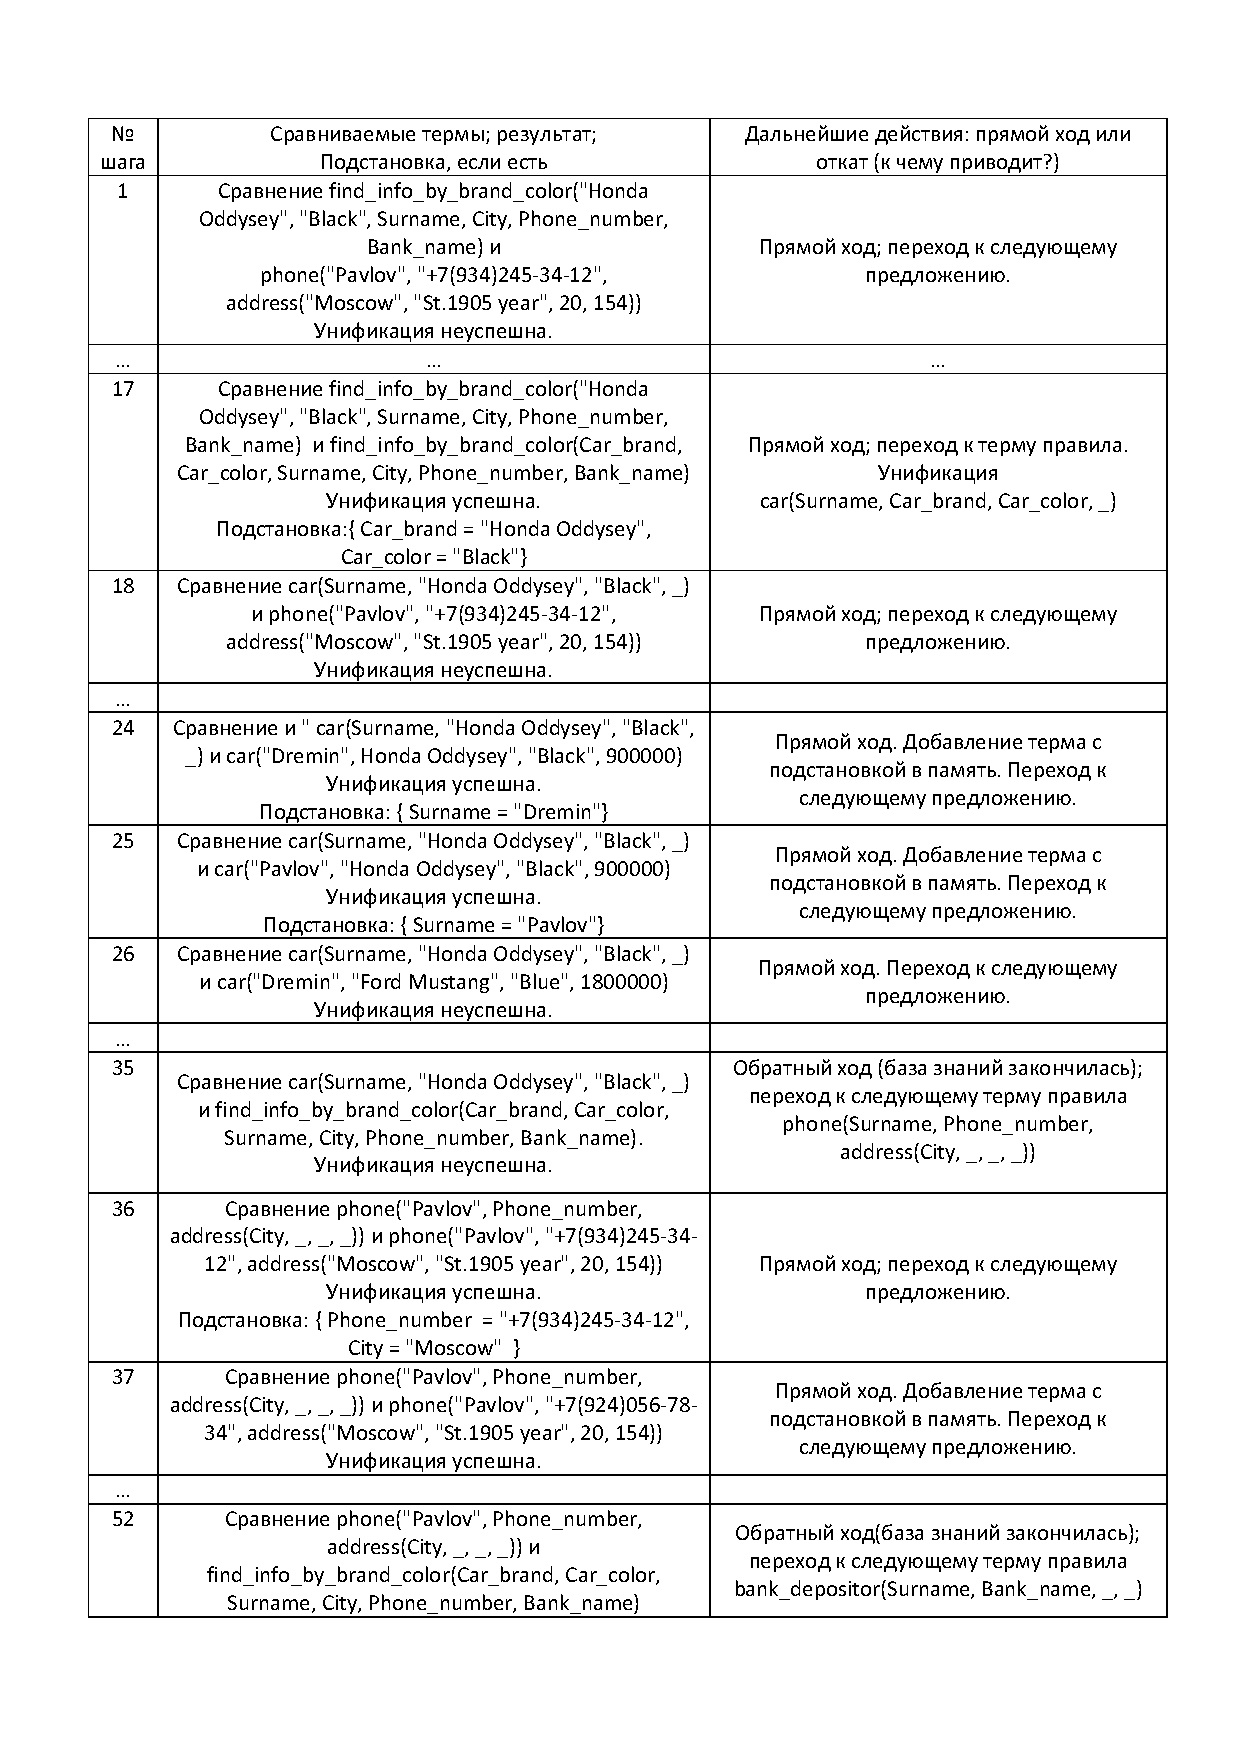
\includegraphics[scale=0.85]{images/table_2_5.pdf}
		\caption{Таблица порядка поиска ответов для задания 2 первый случай.}
		\label{png:1}}
\end{figure}

\begin{figure}[H]
	\centering{
		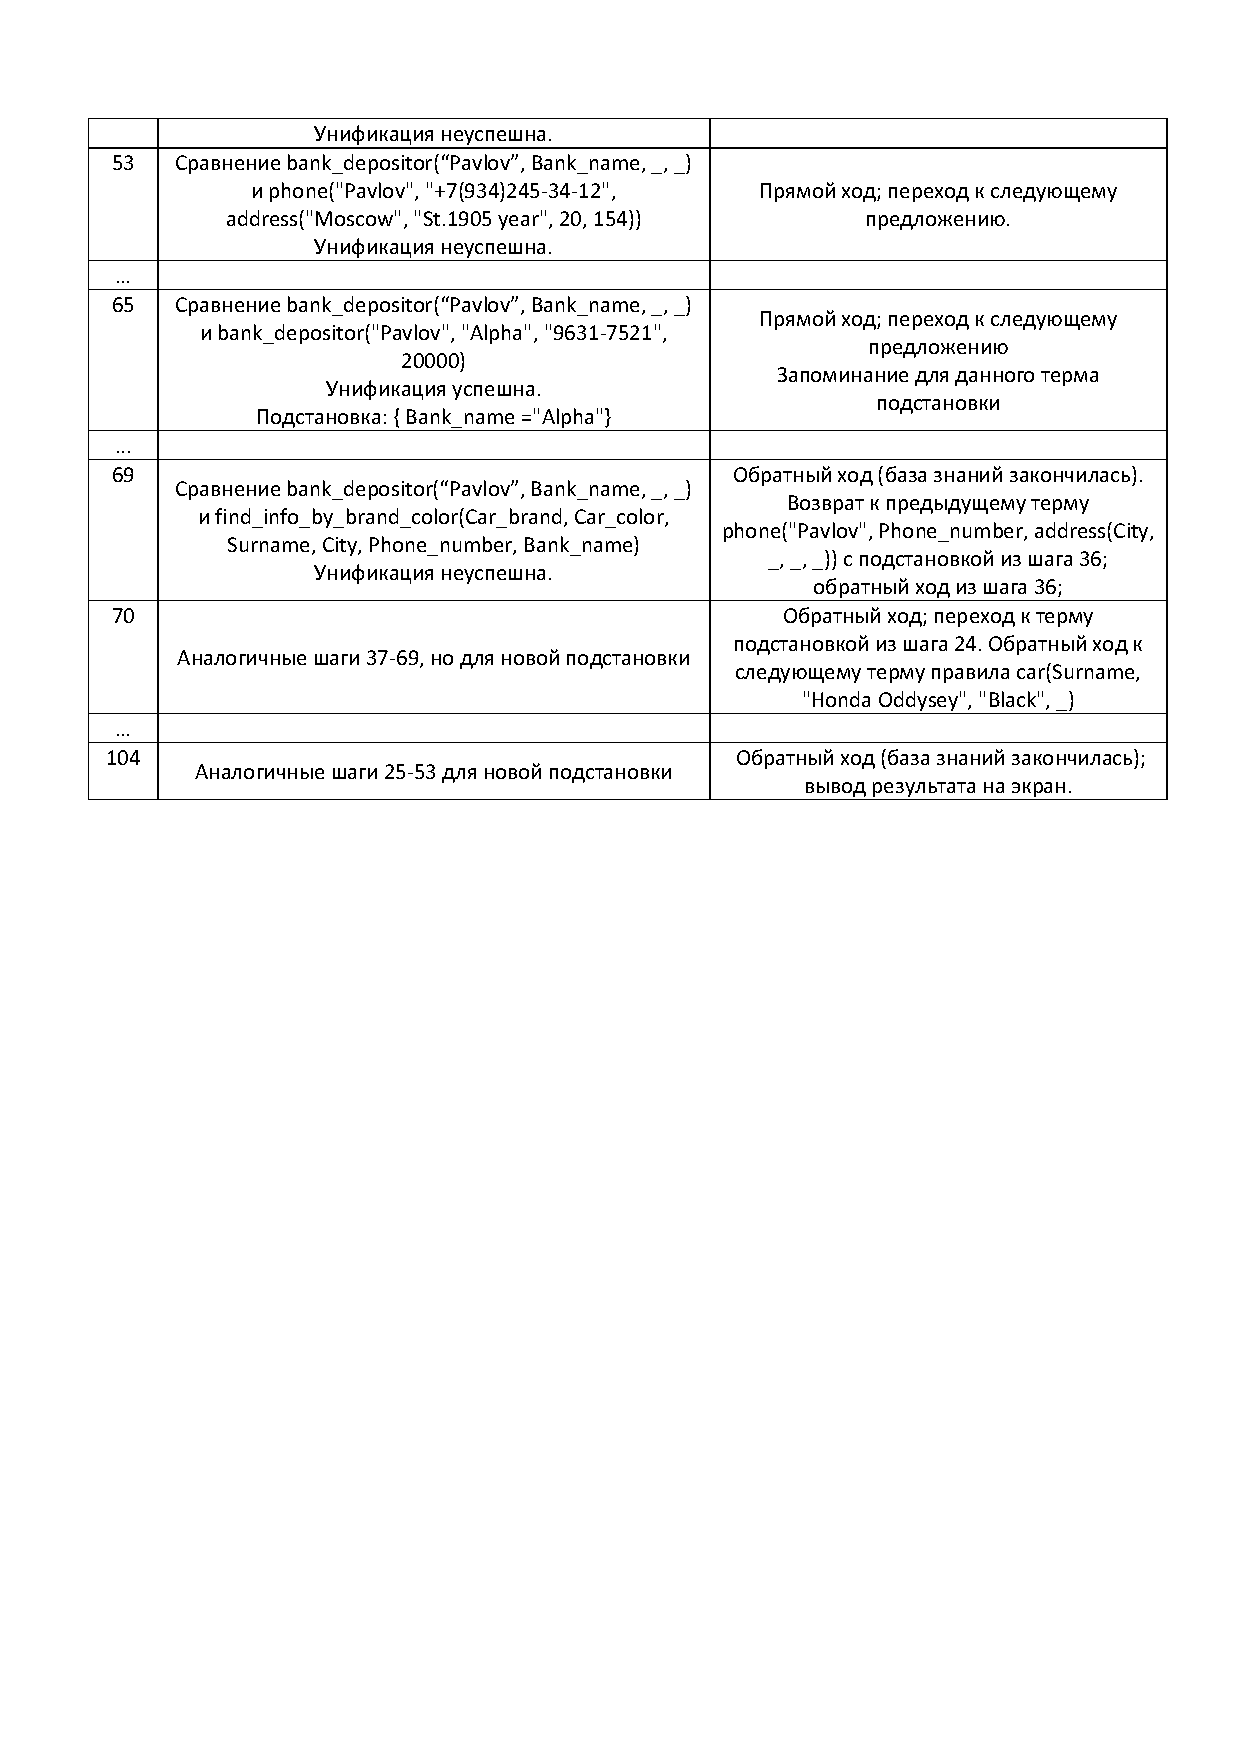
\includegraphics[scale=0.85]{images/table_2_6.pdf}
		\caption{Таблица порядка поиска ответов для задания 2 первый случай (продолжение).}
		\label{png:1}}
\end{figure}

\begin{figure}[H]
	\centering{
		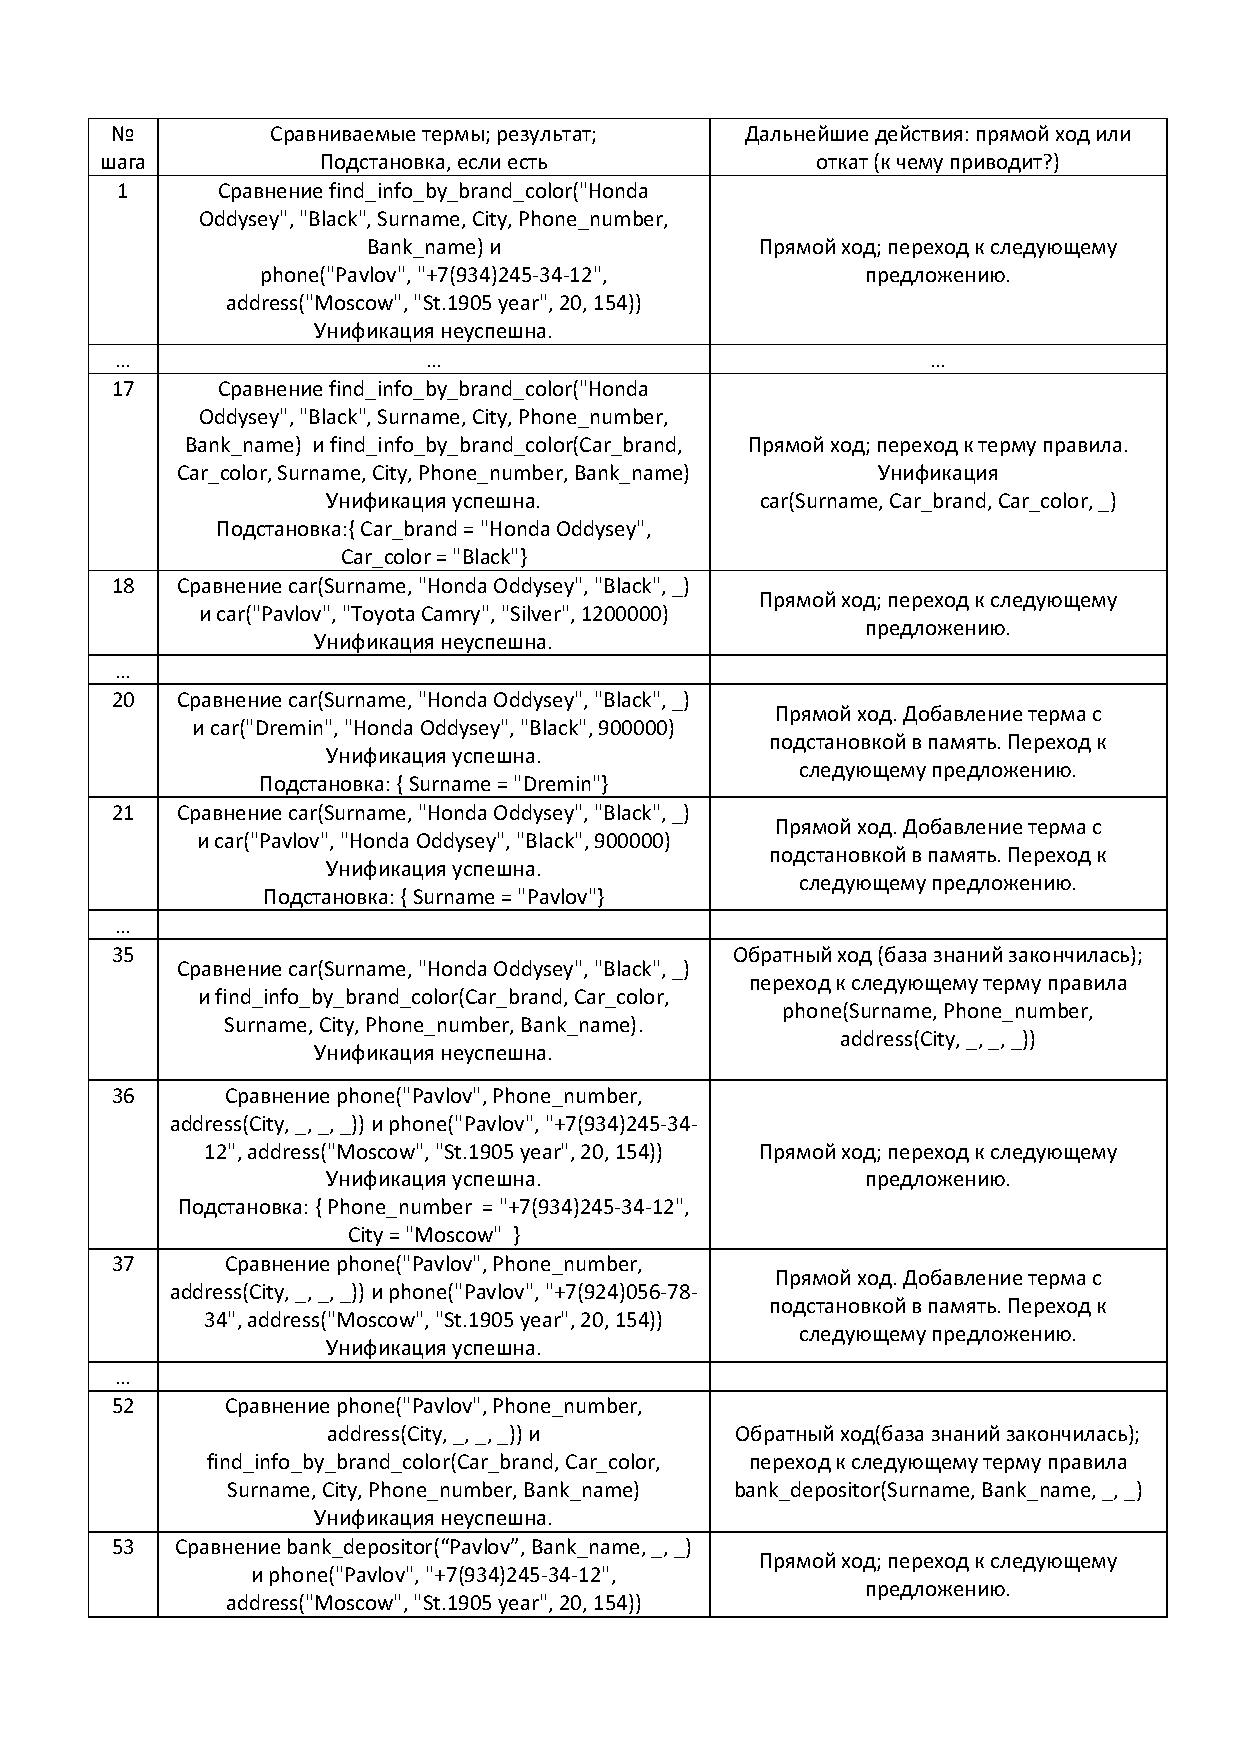
\includegraphics[scale=0.85]{images/table_2_7.pdf}
		\caption{Таблица порядка поиска ответов для задания 2 второй случай (продолжение).}
		\label{png:1}}
\end{figure}

\begin{figure}[H]
	\centering{
		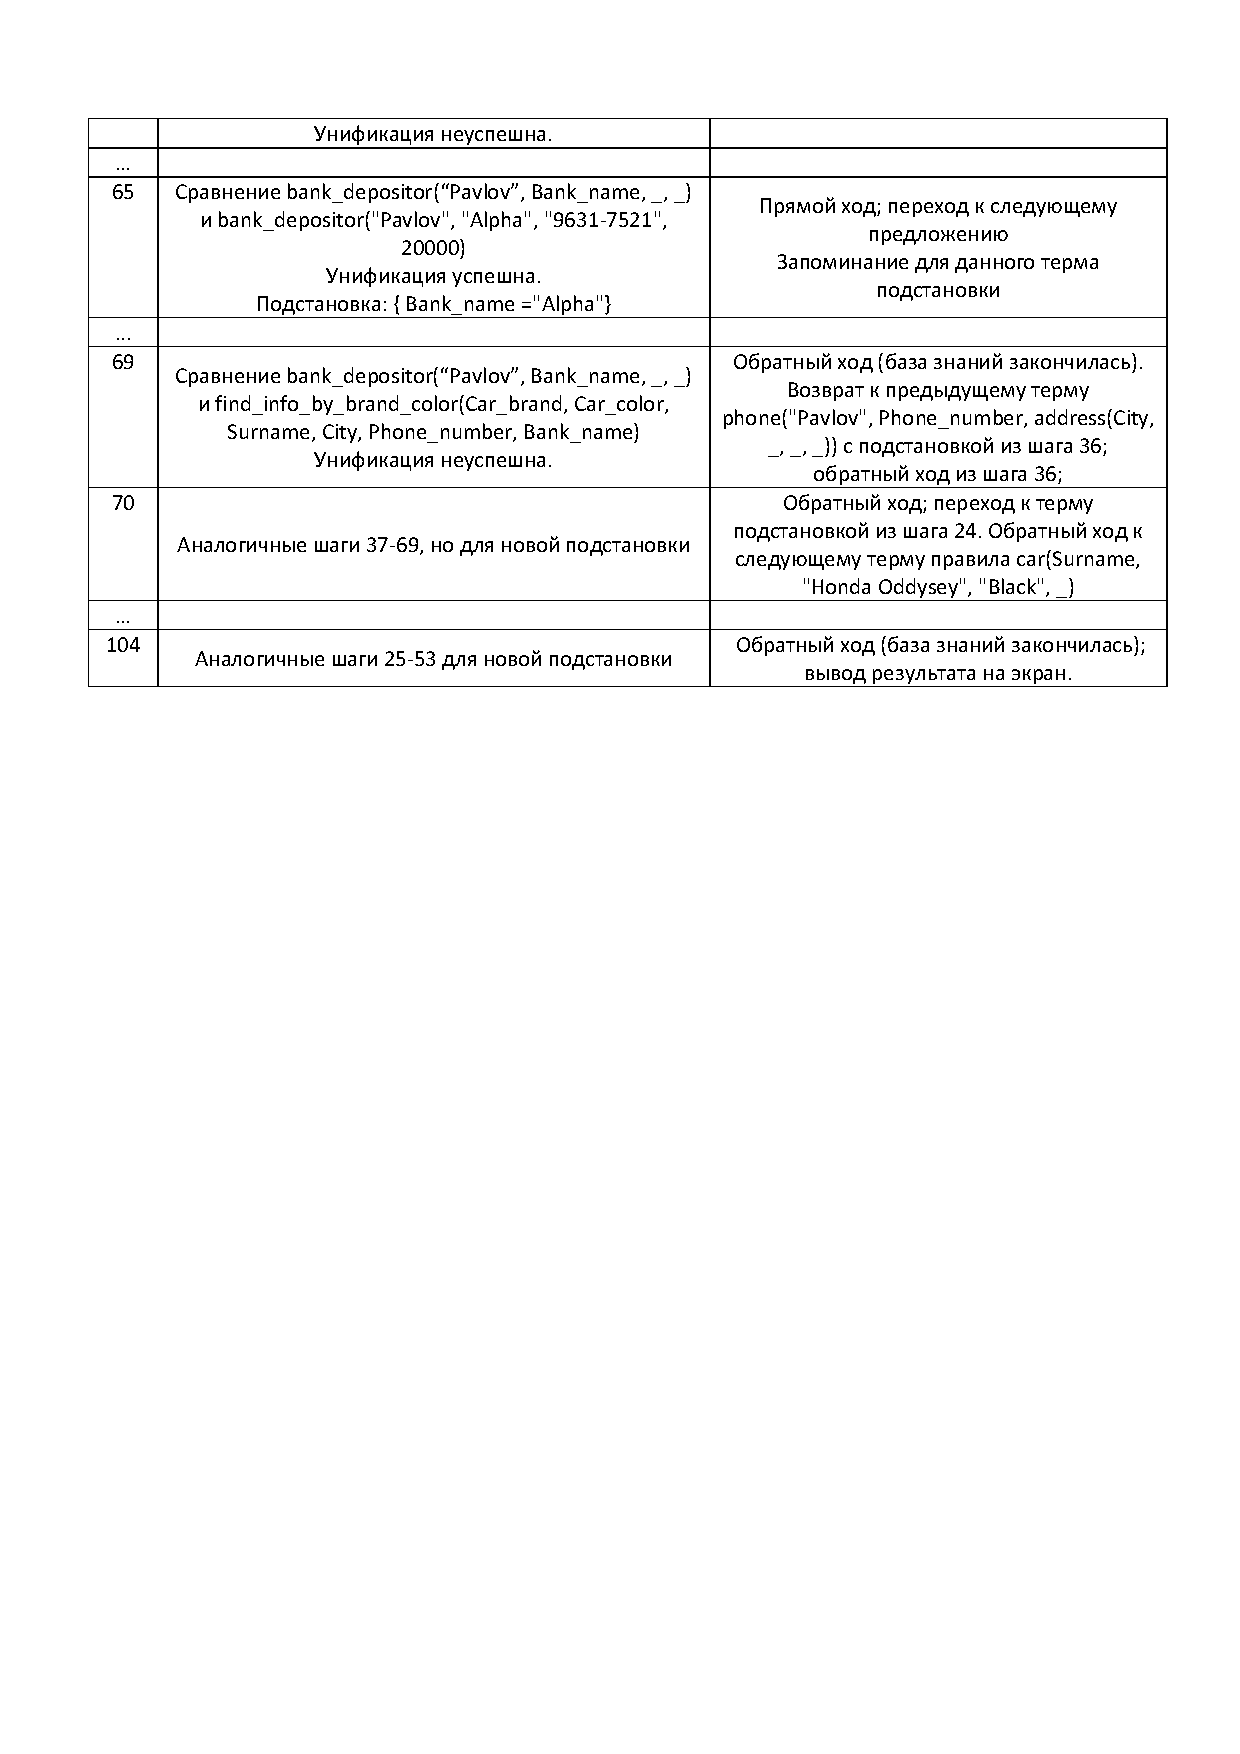
\includegraphics[scale=0.85]{images/table_2_8.pdf}
		\caption{Таблица порядка поиска ответов для задания 2 второй случай (продолжение).}
		\label{png:1}}
\end{figure}
